\documentclass[11pt]{article}
\usepackage[textwidth=18.0cm, textheight=23.0cm, top=2.0cm]{geometry}
\usepackage{pst-all}
\usepackage{amssymb}
\usepackage{tikz}
\usepackage{underscore}\begin{document}
\pagestyle{empty}


ClassName: \underline{\textbf{Class_07.2bp-8}}
\par
BinSize: \underline{\textbf{100 × 100}}
\par
ReduceSize: \underline{\textbf{100 × 99}}
\par
TypeNum: \underline{\textbf{20}}
\par
Num: \underline{\textbf{20}}
\par
OutS: \underline{\textbf{60000}}
\par
InS: \underline{\textbf{48102}}
\par
Rate: \underline{\textbf{0.802}}
\par
UB: \underline{\textbf{6}}
\par
LB0: \underline{\textbf{6}}
\par
LB: \underline{\textbf{6}}
\par
LBWithCut: \underline{\textbf{6}}
\par
NodeCut: \underline{\textbf{0}}
\par
ExtendedNodeCnt: \underline{\textbf{1}}
\par
GenNodeCnt: \underline{\textbf{1}}
\par
PrimalNode: \underline{\textbf{0}}
\par
ColumnCount: \underline{\textbf{6}}
\par
TotalCutCount: \underline{\textbf{0}}
\par
RootCutCount: \underline{\textbf{0}}
\par
LPSolverCnt: \underline{\textbf{1}}
\par
PricingSolverCnt: \underline{\textbf{0}}
\par
BranchAndBoundNum: \underline{\textbf{1}}
\par
isOpt: \underline{\textbf{true}}
\par
TimeOnInitSolution: \underline{\textbf{600.000 s}}
\par
TimeOnPrimal: \underline{\textbf{0.000 s}}
\par
TimeOnPricing: \underline{\textbf{0.000 s}}
\par
TimeOnRmp: \underline{\textbf{0.059 s}}
\par
TotalTime: \underline{\textbf{600.335 s}}
\par
\newpage


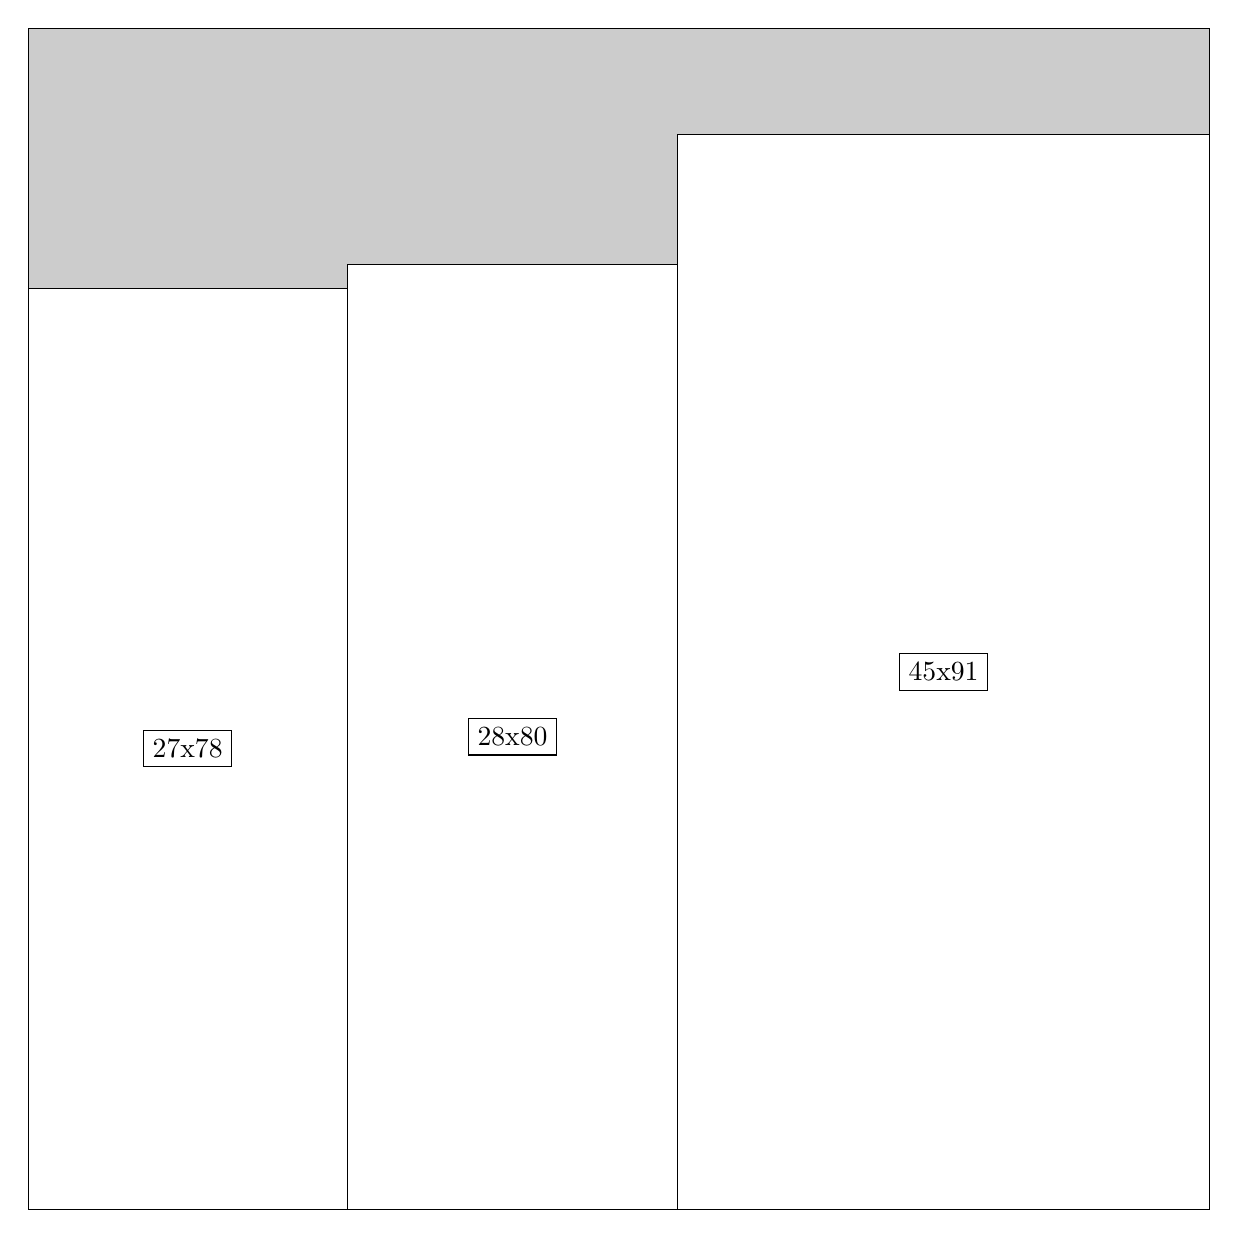
\begin{tikzpicture}[shorten >=1pt,scale=1.0,every node/.style={scale=1.0},->]
\tikzstyle{vertex}=[circle,fill=black!25,minimum size=14pt,inner sep=0pt]
\filldraw[fill=gray!40!white, draw=black] (0,0) rectangle (15.0,15.0);
\foreach \name/\x/\y/\w/\h in {45x91/8.25/0.0/6.75/13.65,28x80/4.05/0.0/4.2/12.0,27x78/0.0/0.0/4.05/11.7}
\filldraw[fill=white!40!white, draw=black] (\x,\y) rectangle node[draw] (\name) {\name} ++(\w,\h);
\end{tikzpicture}


w =45 , h =91 , x =55 , y =0 , v =4095
\par
w =28 , h =80 , x =27 , y =0 , v =2240
\par
w =27 , h =78 , x =0 , y =0 , v =2106
\par
\newpage


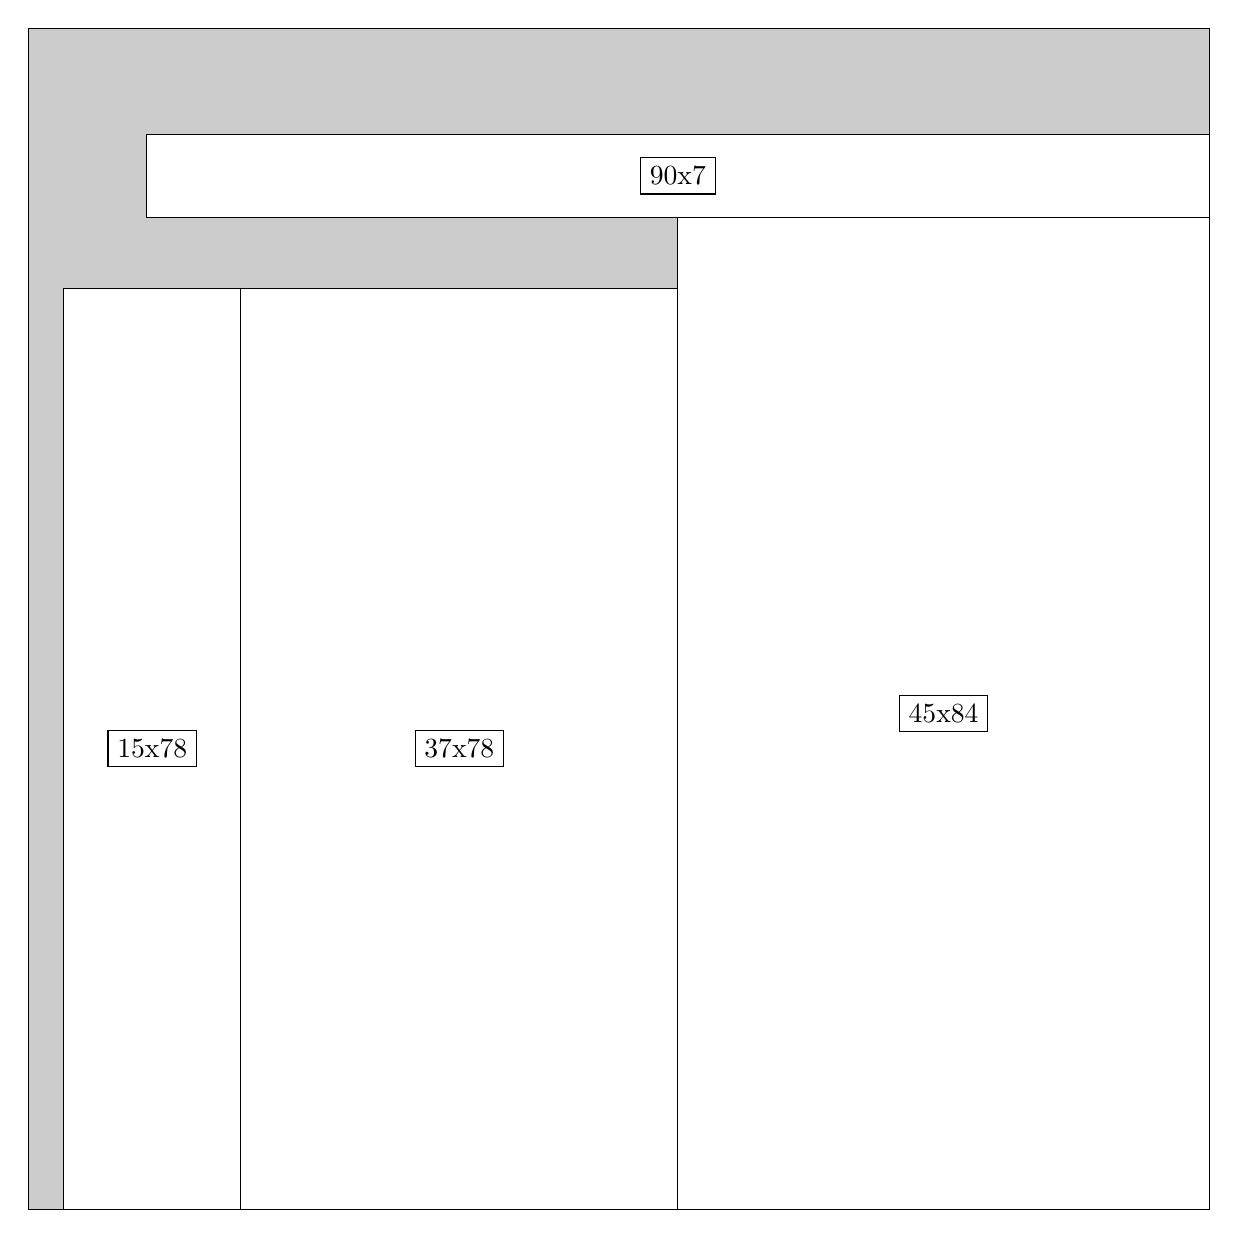
\begin{tikzpicture}[shorten >=1pt,scale=1.0,every node/.style={scale=1.0},->]
\tikzstyle{vertex}=[circle,fill=black!25,minimum size=14pt,inner sep=0pt]
\filldraw[fill=gray!40!white, draw=black] (0,0) rectangle (15.0,15.0);
\foreach \name/\x/\y/\w/\h in {45x84/8.25/0.0/6.75/12.6,37x78/2.6999999999999997/0.0/5.55/11.7,15x78/0.44999999999999996/0.0/2.25/11.7,90x7/1.5/12.6/13.5/1.05}
\filldraw[fill=white!40!white, draw=black] (\x,\y) rectangle node[draw] (\name) {\name} ++(\w,\h);
\end{tikzpicture}


w =45 , h =84 , x =55 , y =0 , v =3780
\par
w =37 , h =78 , x =18 , y =0 , v =2886
\par
w =15 , h =78 , x =3 , y =0 , v =1170
\par
w =90 , h =7 , x =10 , y =84 , v =630
\par
\newpage


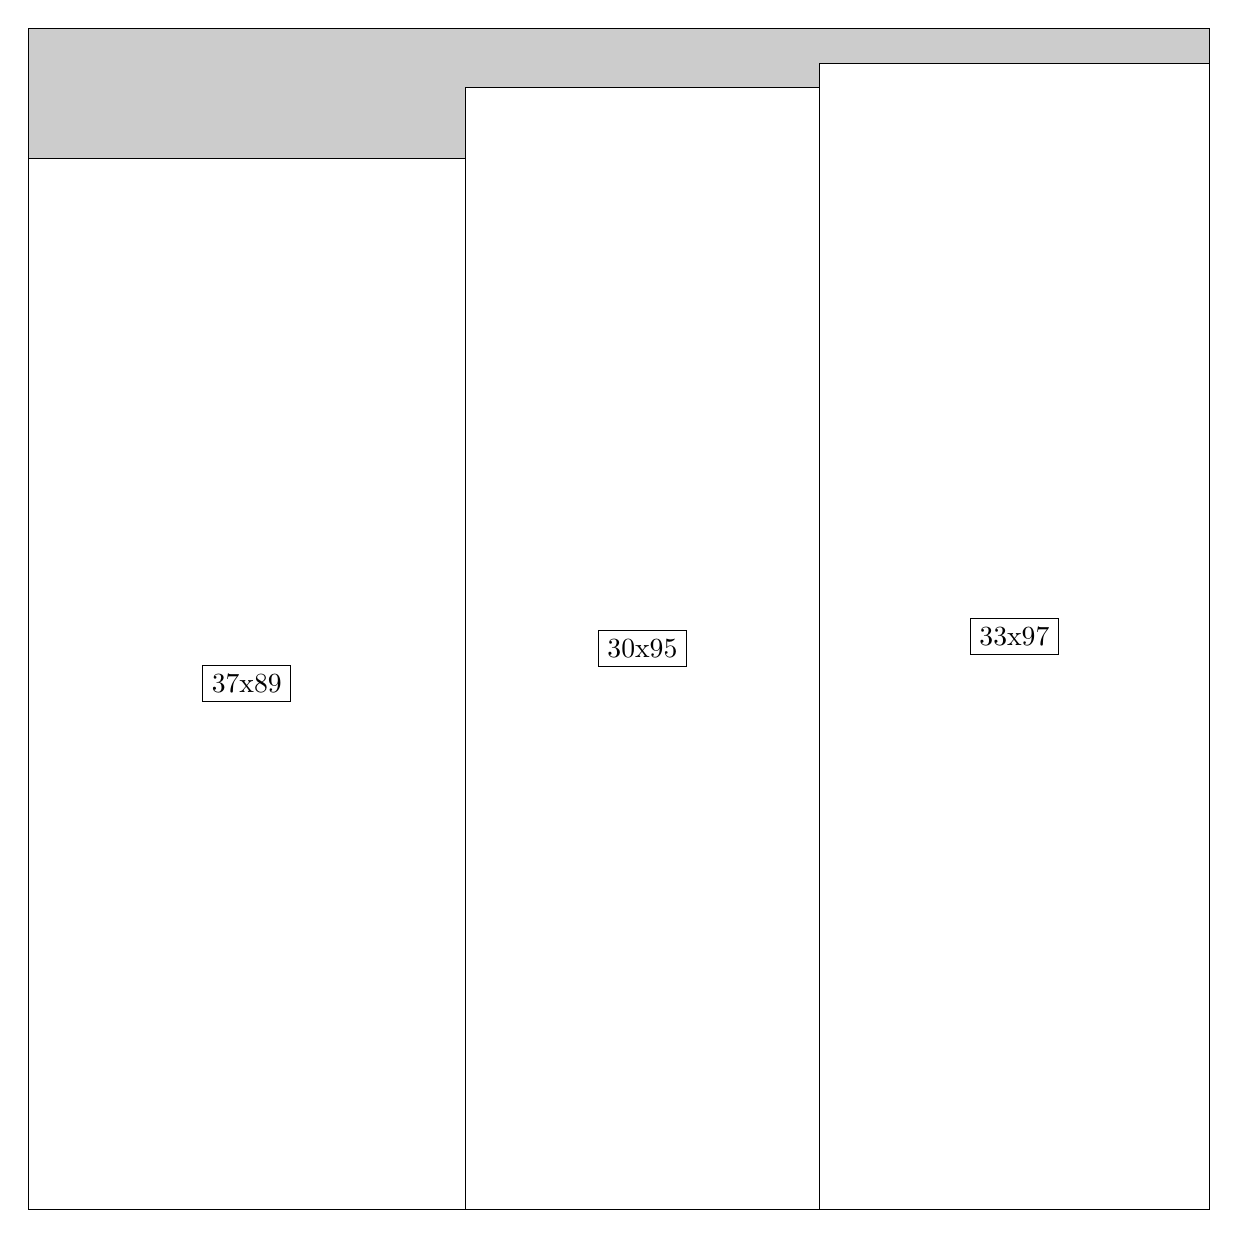
\begin{tikzpicture}[shorten >=1pt,scale=1.0,every node/.style={scale=1.0},->]
\tikzstyle{vertex}=[circle,fill=black!25,minimum size=14pt,inner sep=0pt]
\filldraw[fill=gray!40!white, draw=black] (0,0) rectangle (15.0,15.0);
\foreach \name/\x/\y/\w/\h in {33x97/10.049999999999999/0.0/4.95/14.549999999999999,30x95/5.55/0.0/4.5/14.25,37x89/0.0/0.0/5.55/13.35}
\filldraw[fill=white!40!white, draw=black] (\x,\y) rectangle node[draw] (\name) {\name} ++(\w,\h);
\end{tikzpicture}


w =33 , h =97 , x =67 , y =0 , v =3201
\par
w =30 , h =95 , x =37 , y =0 , v =2850
\par
w =37 , h =89 , x =0 , y =0 , v =3293
\par
\newpage


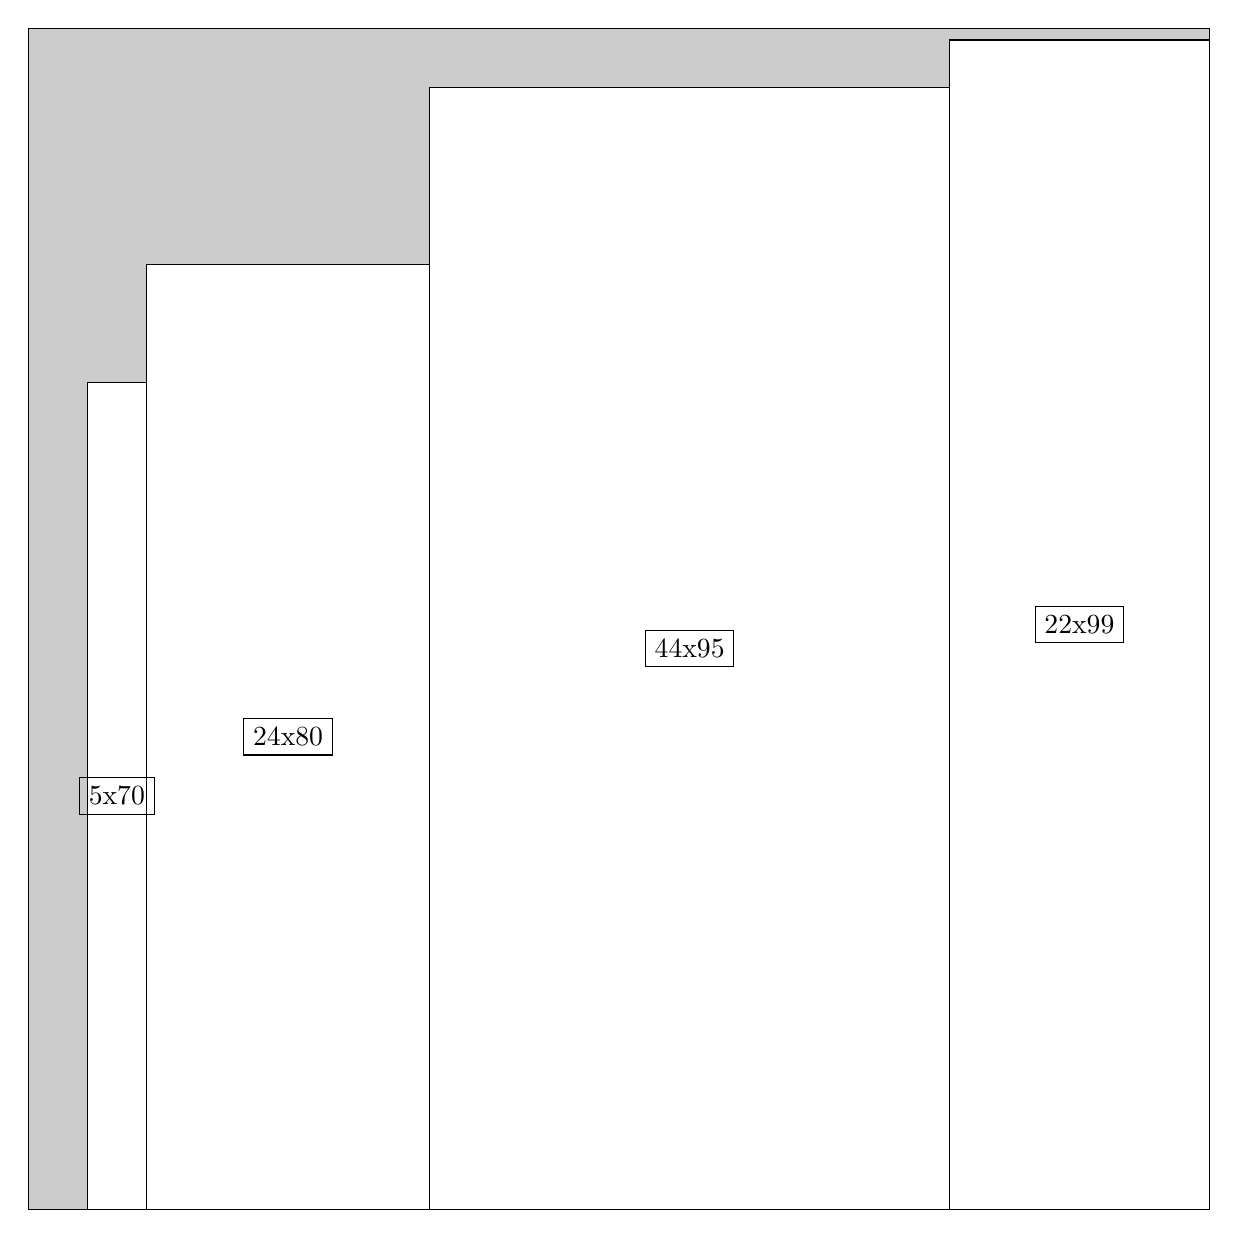
\begin{tikzpicture}[shorten >=1pt,scale=1.0,every node/.style={scale=1.0},->]
\tikzstyle{vertex}=[circle,fill=black!25,minimum size=14pt,inner sep=0pt]
\filldraw[fill=gray!40!white, draw=black] (0,0) rectangle (15.0,15.0);
\foreach \name/\x/\y/\w/\h in {22x99/11.7/0.0/3.3/14.85,44x95/5.1/0.0/6.6/14.25,24x80/1.5/0.0/3.5999999999999996/12.0,5x70/0.75/0.0/0.75/10.5}
\filldraw[fill=white!40!white, draw=black] (\x,\y) rectangle node[draw] (\name) {\name} ++(\w,\h);
\end{tikzpicture}


w =22 , h =99 , x =78 , y =0 , v =2178
\par
w =44 , h =95 , x =34 , y =0 , v =4180
\par
w =24 , h =80 , x =10 , y =0 , v =1920
\par
w =5 , h =70 , x =5 , y =0 , v =350
\par
\newpage


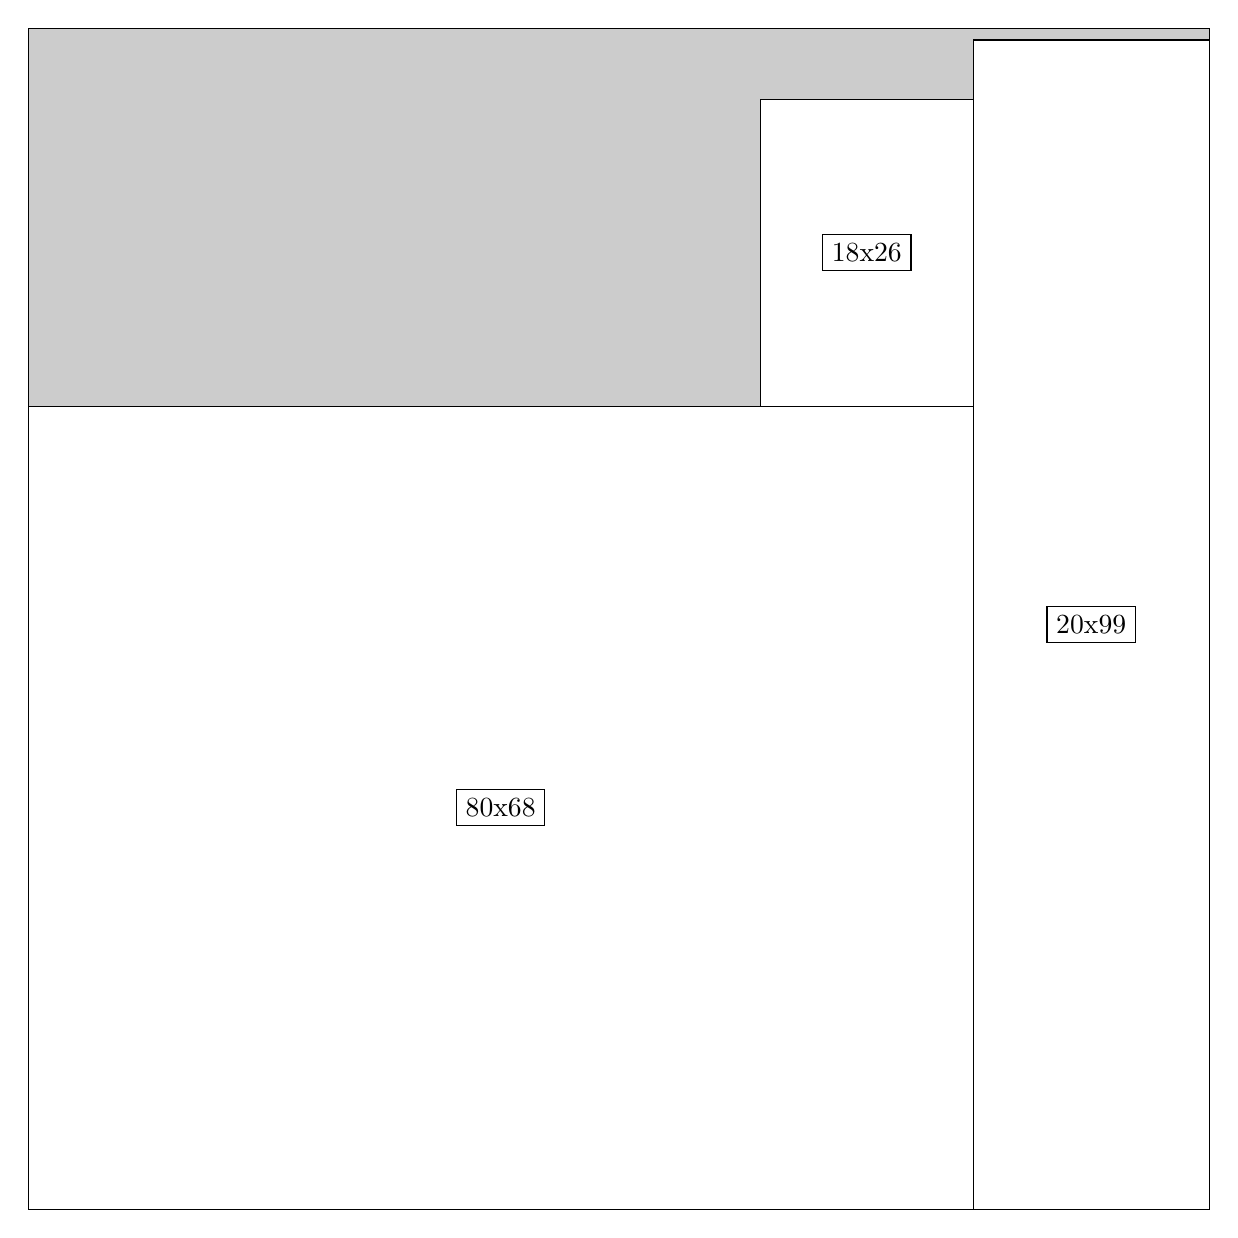
\begin{tikzpicture}[shorten >=1pt,scale=1.0,every node/.style={scale=1.0},->]
\tikzstyle{vertex}=[circle,fill=black!25,minimum size=14pt,inner sep=0pt]
\filldraw[fill=gray!40!white, draw=black] (0,0) rectangle (15.0,15.0);
\foreach \name/\x/\y/\w/\h in {20x99/12.0/0.0/3.0/14.85,80x68/0.0/0.0/12.0/10.2,18x26/9.299999999999999/10.2/2.6999999999999997/3.9}
\filldraw[fill=white!40!white, draw=black] (\x,\y) rectangle node[draw] (\name) {\name} ++(\w,\h);
\end{tikzpicture}


w =20 , h =99 , x =80 , y =0 , v =1980
\par
w =80 , h =68 , x =0 , y =0 , v =5440
\par
w =18 , h =26 , x =62 , y =68 , v =468
\par
\newpage


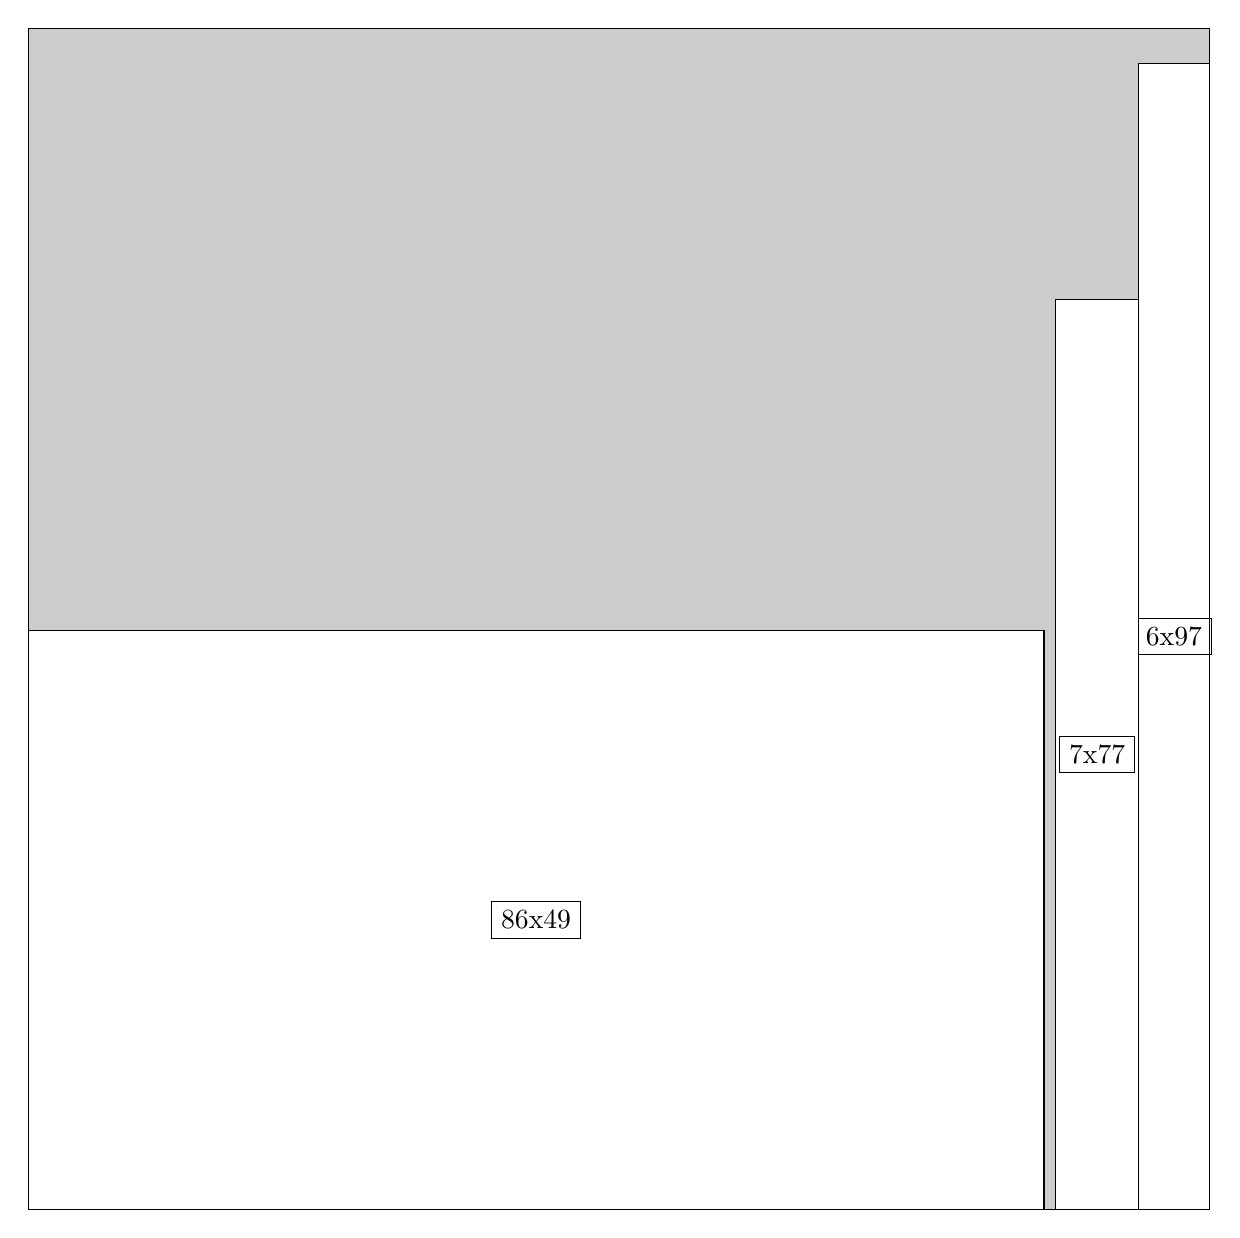
\begin{tikzpicture}[shorten >=1pt,scale=1.0,every node/.style={scale=1.0},->]
\tikzstyle{vertex}=[circle,fill=black!25,minimum size=14pt,inner sep=0pt]
\filldraw[fill=gray!40!white, draw=black] (0,0) rectangle (15.0,15.0);
\foreach \name/\x/\y/\w/\h in {6x97/14.1/0.0/0.8999999999999999/14.549999999999999,7x77/13.049999999999999/0.0/1.05/11.549999999999999,86x49/0.0/0.0/12.9/7.35}
\filldraw[fill=white!40!white, draw=black] (\x,\y) rectangle node[draw] (\name) {\name} ++(\w,\h);
\end{tikzpicture}


w =6 , h =97 , x =94 , y =0 , v =582
\par
w =7 , h =77 , x =87 , y =0 , v =539
\par
w =86 , h =49 , x =0 , y =0 , v =4214
\par
\newpage


\end{document}